% \newcommand\chapternumber{1}
\documentclass[12pt,a4paper]{article}
\usepackage{fullpage}
\usepackage[top=2cm, bottom=4.5cm, left=2.5cm, right=2.5cm]{geometry}
\usepackage{amsmath,amsthm,amsfonts,amssymb,amscd}
\usepackage{lastpage}
\usepackage{enumitem}
\usepackage{fancyhdr}
\usepackage{mathrsfs}
\usepackage{xcolor}
\usepackage{graphicx}
\usepackage{listings}
\usepackage{hyperref}
\usepackage{tikz}
\usetikzlibrary{shapes,backgrounds}
\usepackage[utf8]{inputenc}
\usepackage[ruled, vlined]{algorithm2e}
% \usepackage{apacite}
\usepackage{csquotes}

% Edit these as appropriate
\newcommand\course{Reinforcement Learning}
\newcommand\NetID{sliu1@uvm.edu}
\newcommand\Author{Sida Liu}
\pagestyle{fancyplain}
\headheight 35pt
\lhead{\NetID\\\Author}
% \chead{\textbf{\Large Assignment \chapternumber }}
\rhead{\course \\ \today}
\lfoot{}
\cfoot{}
\rfoot{\small\thepage}
\headsep 1.5em

\setlength{\parskip}{\baselineskip}%
\setlength{\parindent}{0pt}%

\newenvironment{list_abc}
{ \begin{enumerate}[label=(\alph*)] }
{ \end{enumerate} }

\newenvironment{list_iv}
{ \begin{enumerate}[label=\roman*.] }
{ \end{enumerate} }

\hypersetup{
    colorlinks=true,
    linkcolor=blue,
    filecolor=magenta,      
    urlcolor=cyan,
}

\usepackage{tcolorbox}
\usepackage{booktabs}


\begin{document}

\section{Learning Optimization:\\ RL-based Optimizers for Gradient Descent}

\subsection{Structure}
The deliverable will be a piece of open-source software.

\subsection{Topic}
Reinforcement Learning (RL) was developed in the 90s.
The recent boost of RL was benefited from the development of Deep Learning (DL), especially the backpropagation and sophisticated optimization algorithms based on Gradient Descent (GD).
However, currently used optimizers, such as Adam, are still made of hand-designed rules.
It might be possible to produce optimizers that are more adaptive in complex tasks.

In this work, I will propose RL-based Optimizers. We can call them AlphaOpts.
There will be two loops in this design: the outer loop is the Deep Learning task we want to solve; the inner loop is an RL algorithm inside the AlphaOpt.

\begin{figure}[h]
    \center
    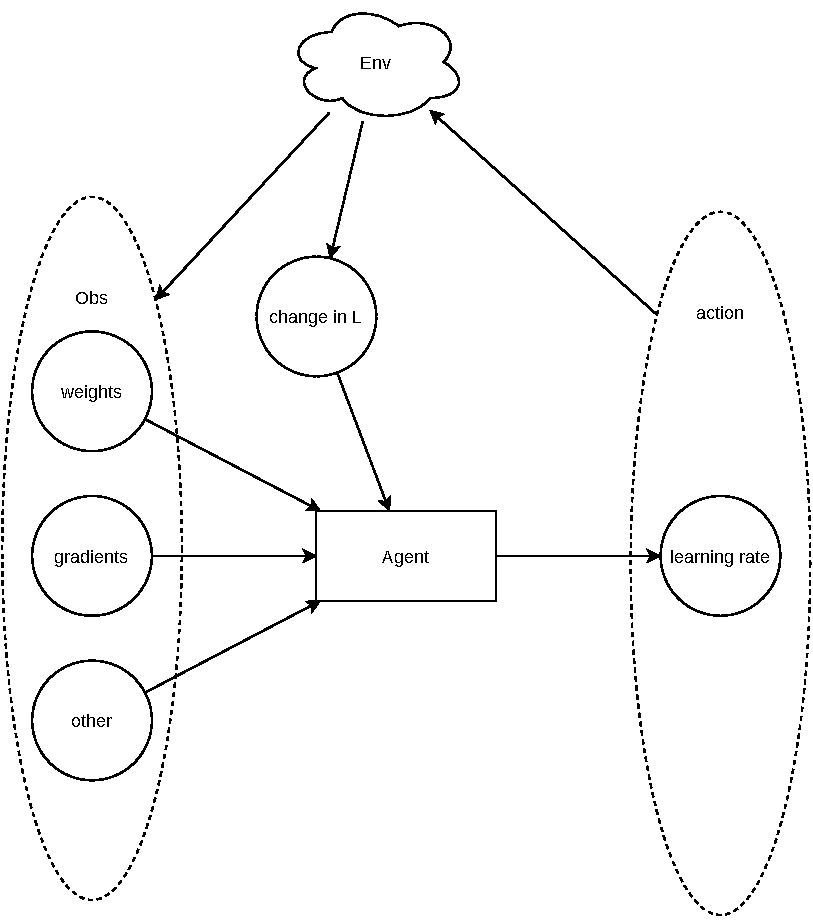
\includegraphics[width=0.5\textwidth]{images/AlphaOpt.pdf}
    \caption{The outer loop of an AlphaOpt}
\end{figure}

The core of an AlphaOpt is a standard Deep RL agent.
The goal of an AlphaOpt is to minimize loss function as fast as possible, $\min_{\theta'} \mathcal{L}$, where $\theta'$ is the inner parameters.
The reward function is the change of the value of the loss function, $-\Delta \mathcal{L}$.
The observation includes current outer parameters, $\theta$, outer gradients, $\nabla_{\theta} \mathcal{L}$, and optionally, other additional information.
The action will be the learning rate for each parameter at that step, $\alpha_\theta$.

Though it is possible to use recursive AlphaOpts, in this work, an AlphaOpt itself will use conventional optimizers, such as Adam, to adjust its parameters.

\subsection{Plan}
The basic principle is \emph{Dream big, Start small}.

\subsubsection{2-D task}
The first task will be a toy task. The purpose of this task is to see the AlphaOpt work in action.
In this task, there will be no Deep Learning in the outer loop.

There are only two outer parameters, so we can visualize the parameter landscape. 
Those landscapes are hand-designed, such as a convex landscape as the simplest case.
We can see the learning process of the AlphaOpt and eventually the parameters of the outer loop reached the minimum.

\subsubsection{MNIST}
The second task is to recognize MNIST hand-written digits.
This is a well-known scenario that we can use a CNN architecture.

I will modify an existing algorithm, replacing the optimizer with an AlphaOpt, and see if it can solve the problem.

\subsubsection{Omniglot}
The third task is to recognize Omniglot letters in a meta-learning setting.
There are many sub-dataset in Omniglot. Our learning algorithm will first train on the meta-training set, and then test on the meta-testing set.
During meta-training, the outer parameters and the inner parameters can change, but during meta-testing, only outer parameters can change, and the inner parameter of AlphaOpts will keep the same.
Thus we can see how a pre-trained optimizer can facilitate the few-shot learning in this setting.

\subsection{Comparison between RL and RNN}
Before I read these two papers, I thought there's little in common between RL and RNN.
However, when I look at these two approaches of making learned optimizers to replace hand-designed optimizer such as Adam, it is very interesting two papers formulate this problem in different ways.
One views the optimizer as an RL agent, and the other views the optimizer as an RNN network.
From this comparison, I learned that RL is a good tool to estimate value function when the gradients are not directly available, for example, a robot can't get gradients directly from the world, so RL can turn the goal (reward function) into estimation and into gradients for the networks.
However, in this case, RNN won, because the optimizer is situated inside the agent, so direct gradients are available, and the optimizer can be viewed as an RNN and apply gradients to update its weights directly.
So, to me, in my hierarchical networks, there will be no need to construct multiple RL agents.

\subsubsection{Learning to Optimize}
\href{https://bair.berkeley.edu/blog/2017/09/12/learning-to-optimize-with-rl/}{https://bair.berkeley.edu/blog/2017/09/12/learning-to-optimize-with-rl/}

Li et al. proposed this idea in 2016 \cite{li2016learning}, which is very similar to my idea.
In Li et al., 2016, the observation contains: (1) Current parameters, $\theta$, (2) The $\Delta \mathcal{L}$ in recent $H$ time steps, (3) The $\nabla_{\theta} \mathcal{L}$ in recent $H$ time steps. (I changed the notation to be aligned with this document.)
The action contains: (1) the update steps, $\Delta \theta = \alpha \nabla_{\theta} \mathcal{L}$.
The goal is to minimize the total area under the learning curve at meta-test time.
The reward function (cost function) is the negative value of outer loss function, $- \mathcal{L}$.
They chose Guided Policy Search (GPS) as the RL algorithm for the optimizer.

Li et al. 2017 provide more details on implementation \cite{li2017learning}, though source code is not available.
The learned optimizer was then tested on several image datasets, which outperforms Adam, AdaGrad, RMSprop in the experiments.

In general, I think Li's implementation can be improved somehow. 
At least I should be able to produce a reusable package that can be easily used in PyTorch.

\subsubsection{Learning to learn by gradient descent by gradient descent}
In contrast, Andrychowicz et al. 2016\cite{andrychowicz2016learning} formulate the optimizer as an RNN neural network.
At every time step, the current parameters $\theta$, and the gradients $\nabla_\theta \mathcal{L}$ are the input to the RNN, along with the hidden state $h_{t-1}$ of the last step.
Just like the RL model, the RNN also produces the update steps, $\Delta \theta$, and the outer network applies the update steps.
Critically, because the whole model is differentiable, so they can directly compute gradients for the RNN optimizer from that step.

Also, to reduce the requirement of memory and make the model more flexible, the RNN model doesn't take concatenated parameters and gradients but take one parameter and one gradient at a time, so all parameters from outer networks pass through the RNN model, producing multiple hidden states and the update steps for their corresponding parameters, respectively.


\bibliographystyle{unsrt}
\bibliography{reference.bib}


\end{document}
